\documentclass[conference]{IEEEtran}
\usepackage{graphicx,amsmath,amssymb,listings,xcolor,url,float}
\usepackage{tikz}
\usetikzlibrary{arrows.meta,positioning,shapes.geometric,shapes.multipart,calc,fit,decorations.pathreplacing}
\usepackage[hidelinks]{hyperref}
\usepackage{iftex}
\ifXeTeX % local tectonic/XeLaTeX build only; Overleaf's pdfLaTeX uses IEEEtran's Times directly
  \usepackage{fontspec}
  \setmainfont{texgyretermes}[Extension=.otf,UprightFont=*-regular,BoldFont=*-bold,ItalicFont=*-italic,BoldItalicFont=*-bolditalic]
  \setmonofont{texgyrecursor}[Extension=.otf,UprightFont=*-regular,BoldFont=*-bold,ItalicFont=*-italic,BoldItalicFont=*-bolditalic]
\fi

\lstset{language=Java,basicstyle=\ttfamily\scriptsize,columns=fullflexible,keepspaces=true,
  frame=single,framesep=2pt,xleftmargin=3pt,xrightmargin=3pt,showstringspaces=false,
  keywordstyle=\bfseries,commentstyle=\itshape\color{black!60},aboveskip=4pt,belowskip=4pt,breaklines=true}

\tikzset{
  flow/.style={-{Stealth[length=4pt]},semithick},
  term/.style={draw,rounded corners=7pt,fill=green!15,minimum height=0.5cm,minimum width=1.4cm,font=\scriptsize},
  proc/.style={draw,fill=pink!40,align=center,text width=3.3cm,minimum height=0.5cm,font=\scriptsize},
  dec/.style={draw,diamond,aspect=2.6,fill=yellow!20,align=center,inner sep=0.5pt,font=\scriptsize},
  alarm/.style={draw,fill=red!25,align=center,text width=3.3cm,minimum height=0.5cm,font=\scriptsize},
  lbl/.style={font=\scriptsize,inner sep=1pt}}

\begin{document}

\title{Observability-Aware Trust-Based Grayhole Detection for Underwater Acoustic Networks}

\author{
\IEEEauthorblockN{Appaji Nagaraja Dheeraj, Aryan Bokolia, and Karthikeya Gupta}
\IEEEauthorblockA{\textit{Department of Computer Science and Engineering} \\
\textit{National Institute of Technology Karnataka, Surathkal}\\
Mangalore, India \\
\{appajidheeraj.241cs110, aryanbokolia.241cs111, karthikeyagupta.241cs117\}@nitk.edu.in}
}

\maketitle

\begin{abstract}
Underwater networks provide new possibilities that can greatly improve our ability to observe and protect the oceans. Underwater acoustic sensor networks are frequently deployed in remote and unattended waters, making them vulnerable to various security threats. Applications based on these networks, such as pollution monitoring, offshore infrastructure inspection and coastal surveillance to name a few, require reliable delivery of every measurement. Various routing protocols have been developed to carry this data over several hops to a surface sink. However, these protocols often place a low priority on security, and a compromised relay that silently drops part of the traffic, known as a grayhole, can degrade the entire network. The classic watchdog defence cannot tell such a relay apart from an honest one whose forwards were lost to collisions, half-duplex deafness or long acoustic links, and it ends up accusing honest nodes. This paper takes a look at the grayhole attack, examines a model of the attack as well as an observability-aware, trust-based detection mechanism created in UnetStack, and compares it with a fixed-threshold watchdog and a channel-aware detector.
\end{abstract}

\begin{IEEEkeywords}
Underwater acoustic sensor network(UASN), Grayhole attack, Selective Forwarding(SF), Trust, Watchdog, UnetStack
\end{IEEEkeywords}

\section{Introduction}

\subsection{Basics of Underwater Acoustic Sensor Networks}
Underwater acoustic sensor networks are now emerging as a hot topic among researchers due to a surge of novel applications in ocean sampling, environmental monitoring, offshore exploration, disaster prevention and tactical surveillance. An Underwater Acoustic Sensor Network (UASN) consists of sensors placed under water that sense the environment and communicate using sound, since radio waves are absorbed within a few metres of sea water. Each device that can send, receive and relay data is called a \emph{Node}. One special node, the \emph{sink}, is usually a surface buoy that collects the data and passes it on to the shore.

Sound travels at about 1500~m/s in water, nearly five orders of magnitude slower than radio. The acoustic channel faces a number of challenges, some of which are given in~\cite{akyildiz}: long and variable propagation delay, low and distance-dependent bandwidth, high bit-error rates, noise from ships, boats and marine life, and nodes that run on batteries that are hard to replace. Moreover, most acoustic modems are half-duplex: a node cannot hear while it is transmitting. A sensor that is far from the sink therefore depends on other nodes to relay its packets hop by hop.

Attackers can use these issues to their advantage. Since packets are lost often even in an honest network, a compromised relay can drop packets without causing much suspicion. Nodes are deployed unattended, so physically capturing one and loading malicious code into it is feasible. Unlike a terrestrial network, there is no cheap way to inspect a node that sits hundreds of metres below the surface.

As a result, security is a major issue faced by UASNs currently. Light-weight detection schemes that do not mistake the channel for an attacker are the need of the hour. This paper looks into detecting the grayhole attack, a form of selective forwarding, at the network layer.

\subsection{Selective Forwarding and the Grayhole Attack}
In a multi-hop network, the role of a routing node is to receive packets from its neighbours and forward them towards the sink. A selective forwarding attack~\cite{karlof} occurs when such a node forwards only some of the packets and drops the rest. When every packet is dropped, the node is called a \emph{blackhole}; it is easy to find, because traffic through it stops completely. A \emph{grayhole} drops only a fraction of the packets, for example 30\%, so its loss blends with the normal loss of the acoustic channel. The attack raises the packet loss rate and lowers the throughput and reliability of every route that passes through the malicious node. Since the busiest relays carry the traffic of many sensors, a single grayhole can affect a large part of the network.

There are 2 ways by which a malicious node can attack the network, as explained in~\cite{karlof,domingo}.
\begin{enumerate}
\item Insider Attack
\item Outsider Attack
\end{enumerate}
An \emph{insider attack} is carried out by a node that belongs to the network and holds its keys, for example a captured sensor running malicious code. Since it takes part in routing legitimately, cryptography alone cannot stop it from dropping packets. An \emph{outsider attack} is carried out by a node that does not belong to the network, for example by jamming or by replaying packets. Outsider attacks can be limited with authentication. The grayhole considered in this paper is an insider.

\subsection{Types of Selective Forwarding}
Selective forwarding appears in several forms~\cite{karlof,jiang}:
\begin{itemize}
\item \textbf{Blackhole:} the node drops every packet that it should forward.
\item \textbf{Grayhole:} the node drops packets with a given probability, or only those of chosen sources, so the loss looks like that of a poor channel.
\item \textbf{On--off attack:} the node behaves well for a while to build trust and then drops packets, repeating the cycle.
\item \textbf{Denial of Service:} the node drops control packets, such as route updates, so that its neighbours lose their routes.
\end{itemize}
There are a variety of solutions available for these attacks, but often these require acknowledgements from every hop, extra probe packets or cryptographic exchanges, which use high amounts of energy and bandwidth. This is a luxury that cannot be afforded in the case of UASNs. Hence, the approach in this paper only listens to traffic that is already sent, and it was chosen taking this and the feasibility of implementation into account.

The rest of the paper is organised as follows: Section~\ref{sec:related} presents a review on various related works of literature. Section~\ref{sec:design} presents the design of the grayhole attack model and the detection approach. Section~\ref{sec:impl} explains the implementation of both in UnetStack. Section~\ref{sec:results} presents results of a performance evaluation done on both implementations, together with a comparison against the baselines. Section~\ref{sec:conclusion} concludes the paper and provides suggestions for future work.

\section{Related Work}\label{sec:related}
The authors of~\cite{akyildiz} elaborate on the architecture of UASNs and the research challenges of every layer, from the slow and lossy acoustic channel up to routing. The paper authored by~\cite{karlof} talks about attacks on routing in sensor networks, and is one of the first to define selective forwarding and to show why it is hard to counter. Domingo in~\cite{domingo} lists the attacks that apply to underwater networks, including selective forwarding, sinkhole and wormhole attacks, and the countermeasures available for each. These papers however only presented general-purpose solutions, and they do not describe how a node should decide that a neighbour is malicious.

The paper by~\cite{jiang} contains an extensive literature survey of security in underwater acoustic networks, covering every layer from the physical layer to the application. It points out that most terrestrial defences assume a reliable channel and cheap communication, neither of which holds under water.

Marti \emph{et al.} in~\cite{marti} introduced the \emph{watchdog}: a node that has sent a packet to its next hop keeps listening, and if it does not overhear the next hop forwarding the packet within a timeout, it counts a miss. A node whose misses exceed a threshold is reported as misbehaving. The method is simple, distributed and needs no extra packets. Some possible drawbacks noticed were, as the authors themselves point out, ambiguous collisions, receiver collisions and partial dropping: a miss can be caused by a collision at the monitor or at the relay, not only by the relay.

Shila \emph{et al.} in~\cite{shila} improve on this for grayhole attacks in wireless mesh networks with a Channel-Aware Detection (CAD) scheme. CAD estimates the normal loss that the channel and medium-access collisions would cause, and accuses a node only when its observed loss is clearly higher than this estimate. It combines upstream and downstream monitoring with probe and acknowledgement packets. Hence, there is a trade-off involved here: better accuracy is paid for with extra control traffic, which is costly under water.

The group who authored~\cite{hanTrust} did another study on trust in UASNs and built a trust model from several metrics, namely link, data and energy trust. Liu \emph{et al.}~\cite{liu} use an adaptive trust evaluation to detect abnormal nodes, and Han \emph{et al.}~\cite{hanRouting} combine trust with fuzzy logic to choose reliable relays in layered underwater routing. These trust models show that trust is useful under water, but they compute trust from counts of successful interactions and do not ask whether a failed interaction could have been observed in the first place.

Chandavarkar and Suresh in~\cite{brc} demonstrated the selective forwarding attack and a detection mechanism in UnetStack3. Their work showed that the attack can be built and studied on an underwater network stack. Of the methods above, the fixed-threshold watchdog of~\cite{marti} is the simplest to implement and is the style of detector used for this demonstration. It is distributed and needs no extra packets. Hence, it was chosen as the baseline of this paper. A CAD-style detector adapted from~\cite{shila} is used as a second comparator. Both comparators are adaptations: our watchdog does not reproduce the destination-timeout details of~\cite{brc}, and our CAD-style detector keeps only the downstream channel and collision estimate of~\cite{shila}. Removing a detected node can consume a lot of energy and can cut off the nodes behind it. Hence, our approach only detects grayholes and routes traffic around them where another path exists.

Most of the work above was tested on general network simulators designed for terrestrial or radio networks. UnetStack~\cite{chitre} is an agent-based network stack and simulator for underwater networks, in which the same agents can run on real modems. There is a dearth of papers covering simulations in UnetStack, especially in the domain of security. This paper seeks to address that by providing one such implementation, built with the physical-layer notifications that UnetStack provides~\cite{unet}.

\section{Design of the Grayhole Attack and its Detection}\label{sec:design}

\subsection{Attack Model}
A 20-node network created on UnetStack is used to demonstrate the attack. Twenty sensors are placed at random positions in a 4~km~$\times$~4~km field on one side of the sink, and the layout is redrawn until every sensor can reach the sink. Every sensor generates data for the sink, and each one sends its packets to the nearest neighbour that is one hop closer to the sink. The three relays that carry the most traffic are made malicious. One of the ten test networks is given in Figure~\ref{fig:topology}.

\begin{figure}[t]\centering
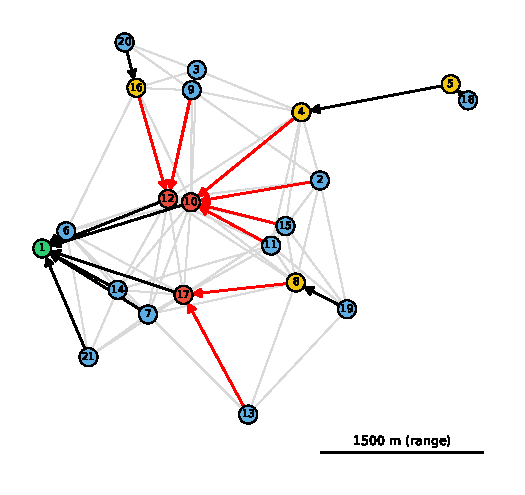
\includegraphics[width=0.95\columnwidth]{figs/topology.pdf}
\caption{Network topology to simulate the grayhole attack (test network 201).}\label{fig:topology}
\end{figure}

In the figure, node 1 is the sink, coloured green. The sensors that only send their own data are coloured blue, the honest relays are coloured yellow and the three grayholes, nodes 10, 12 and 17, are coloured red. The arrows show the route that each node uses towards the sink. The arrows in black are routes into honest nodes, and the arrows in red are routes into a grayhole, along which part of the traffic is dropped. The thin grey lines join nodes that are within the 1500~m communication range of each other; along these lines a node can overhear its neighbour. The scale bar shows the communication range. Nodes 7 and 14 are only about 100~m apart and are drawn slightly apart so that both can be read.

Initially, every node will start sending data packets to its next hop at random times. When a grayhole receives a packet that it should forward, it will draw a random number between 0 and 1. If the number is below the drop probability $p$ (0.3 in most of the experiments), the packet will be dropped silently; otherwise it will be forwarded as usual. The grayhole still sends its own data and still answers every request, so it looks like an honest node to its neighbours. A flowchart showing the course of the program is given in Figure~\ref{fig:attackflow}.

\begin{figure}[t]\centering
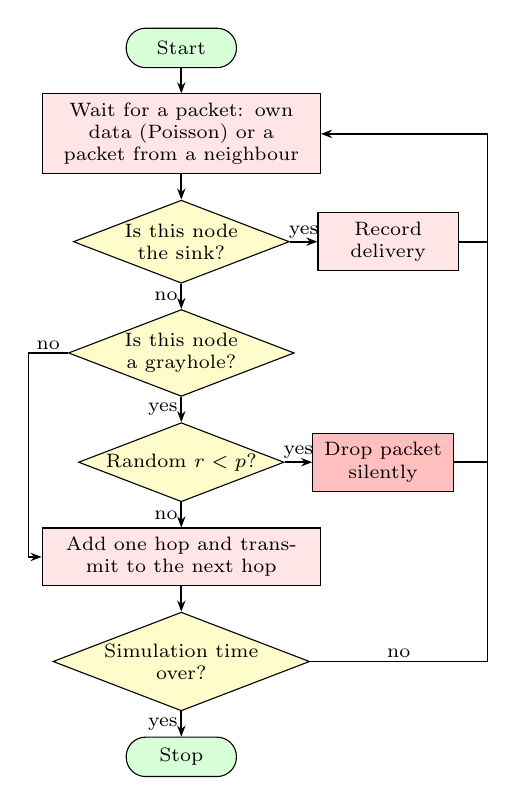
\begin{tikzpicture}[node distance=0.32cm]
\node[term] (s) {Start};
\node[proc,below=of s] (w) {Wait for a packet: own data (Poisson) or a packet from a neighbour};
\node[dec,below=of w] (sink) {Is this node\\the sink?};
\node[proc,right=0.35cm of sink,text width=1.55cm] (rec) {Record delivery};
\node[dec,below=of sink] (gh) {Is this node\\a grayhole?};
\node[dec,below=of gh] (r) {Random $r < p$?};
\node[proc,right=0.35cm of r,text width=1.55cm,fill=red!25] (drop) {Drop packet silently};
\node[proc,below=of r] (fw) {Add one hop and transmit to the next hop};
\node[dec,below=of fw] (t) {Simulation time\\over?};
\node[term,below=of t] (e) {Stop};
\draw[flow] (s)--(w); \draw[flow] (w)--(sink);
\draw[flow] (sink)--node[lbl,above]{yes}(rec);
\draw[flow] (sink)--node[lbl,left]{no}(gh);
\draw[flow] (gh)--node[lbl,left]{yes}(r);
\draw[flow] (gh.west)--node[lbl,above]{no}++(-0.5,0)|-(fw.west);
\draw[flow] (r)--node[lbl,above]{yes}(drop);
\draw[flow] (r)--node[lbl,left]{no}(fw);
\draw[flow] (fw)--(t);
\draw[flow] (t)--node[lbl,left]{yes}(e);
\coordinate (L) at ($(t.east)+(2.25,0)$);
\draw[flow] (t.east)--node[lbl,above]{no}(t.east-|L)|-(w.east);
\draw[semithick] (rec.east)--(rec.east-|L);
\draw[semithick] (drop.east)--(drop.east-|L);
\end{tikzpicture}
\caption{Sequence of the attack model.}\label{fig:attackflow}
\end{figure}

\subsection{Detection Approach}
The detection approach starts from the watchdog of~\cite{marti}, which is the baseline of this paper. It is distributed: every node that sends a packet watches its own next hop. The following rules are followed by each monitor node:

\textbf{Rule 1:} \emph{After sending a packet to the next hop, listen for its forward; a forward that is not heard in time is a miss.}

\textbf{Rule 2:} \emph{If the fraction of misses exceeds a fixed threshold (30\%), accuse the next hop.}

Given in Figure~\ref{fig:baseline} is the algorithm of the baseline watchdog.

\begin{figure}[t]
\begin{lstlisting}
Repeat
  send packet P to next hop B; sent[B]++
  start timer for P
  if (forward of P by B overheard before timeout)
    // B behaved well for P
  else
    miss[B]++                // any silence counts
  if (sent[B] >= MIN_OBS && miss[B]/sent[B] > 0.3)
    accuse(B)                // fixed threshold
Until No transmission
\end{lstlisting}
\caption{Baseline fixed-threshold watchdog algorithm (after~\cite{marti}).}\label{fig:baseline}
\end{figure}

In the baseline, every silence is blamed on the next hop. Under water, however, a forward can be missed although the relay is honest: the monitor itself was transmitting and was deaf (half-duplex), the packet collided at the relay so the relay never received it, or the long acoustic link lost the packet or its forward. These losses grow with traffic, so with a fixed threshold the baseline either accuses honest relays or misses grayholes, and routing around wrongly accused relays forces detours that lower delivery.

Taking into account what an acoustic node in UnetStack can actually observe, the following modifications were made:
\begin{itemize}
\item \textbf{Observability:} every neighbour of a relay watches it, and a watch window counts only if the monitor could have heard the forward. Windows hidden by the monitor's own transmission or by a known collision at the relay are ignored, instead of being counted as misses.
\item \textbf{Trust from the expected loss of each link:} for each link the monitor computes, from the node distances and the normal loss of the link's distance area (near, medium or far), how many forwards an honest relay should show. Trust is the number of forwards heard divided by the number expected, combined over all monitors.
\item \textbf{Dynamic threshold and confirmation:} a relay is flagged only when its shortfall is significant for the current network, and it becomes a suspect only after two flagged rounds in a row. Confirmed grayholes leave the normal-loss baseline, so further grayholes stand out.
\end{itemize}

The timing of one watch is shown in Figure~\ref{fig:window}. Let $M$ be the monitor, $A$ the node that sent packet $P$ and $B$ the relay. From the known positions and the speed of sound $c$, $M$ works out when $P$ was arriving at $B$ (interval $I_B$) and when $B$'s forward should reach $M$ (window $W$). $W$ is as long as the forward allowance of 2~s plus one frame.

\begin{figure}[t]\centering
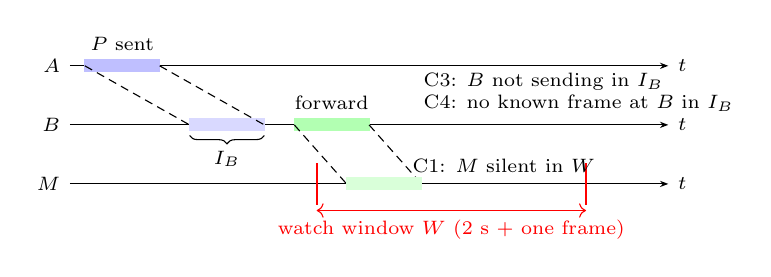
\begin{tikzpicture}[x=0.95cm,y=0.75cm,font=\scriptsize]
\foreach \y/\n in {2/A,1/B,0/M} {\draw[-{Stealth[length=3pt]}] (0,\y)--(8,\y) node[right]{$t$}; \node[left] at (0,\y) {$\n$};}
\fill[blue!25,draw] (0.2,1.9) rectangle (1.2,2.1); \node[above] at (0.7,2.1) {$P$ sent};
\fill[blue!15,draw] (1.6,0.9) rectangle (2.6,1.1);
\draw[densely dashed] (0.2,2)--(1.6,1); \draw[densely dashed] (1.2,2)--(2.6,1);
\draw[decorate,decoration={brace,amplitude=3pt,mirror}] (1.6,0.82)--(2.6,0.82) node[midway,below=2pt]{$I_B$};
\fill[green!30,draw] (3.0,0.9) rectangle (4.0,1.1); \node[above] at (3.5,1.1) {forward};
\draw[densely dashed] (3.0,1)--(3.7,0); \draw[densely dashed] (4.0,1)--(4.7,0);
\fill[green!15,draw] (3.7,-0.1) rectangle (4.7,0.1);
\draw[red,thick] (3.3,-0.35)--(3.3,0.35); \draw[red,thick] (6.9,-0.35)--(6.9,0.35);
\draw[red,<->] (3.3,-0.45)--node[below]{watch window $W$ (2 s + one frame)}(6.9,-0.45);
\node[align=left,anchor=west] at (4.6,1.55) {C3: $B$ not sending in $I_B$\\C4: no known frame at $B$ in $I_B$};
\node at (5.8,0.3) {C1: $M$ silent in $W$};
\end{tikzpicture}
\caption{Watch window of monitor $M$ for relay $B$. Dashed lines show propagation at 1500~m/s.}\label{fig:window}
\end{figure}

A window is kept only if three conditions hold. \textbf{C1:} $M$ did not transmit during $W$. \textbf{C3:} $M$ did not hear $B$ transmitting while $P$ was arriving at $B$, since $B$ was then deaf. \textbf{C4:} no frame known to $M$, whether its own or one it decoded from another neighbour, reached $B$ during $I_B$, so $P$ did not collide at $B$. The same conditions are applied to heard and missed forwards. A fourth candidate, a corrupted frame at $M$ (C2), is deliberately not used, because the relay's own forward can cause it while a drop never does: excluding such windows would remove honest forwards more often than drops.

For each kept window, the chance that an honest forward reaches $M$ through the channel alone is $g=(1-e(d_{AB}))(1-e(d_{BM}))$, where $e(d)=0.15\,(d/1500)^2$ is the frame loss at distance $d$. The loss that the channel does not explain, mainly collisions, is learned from the network itself: for each distance area it is the median loss of the \emph{other} relays' links, so the relay being judged cannot hide in its own baseline. The expected forwards on a link are then $E=G(1-\kappa_{\mathrm{area}})$, where $G$ is the sum of $g$ over its windows. The trust of relay $B$ is the total heard divided by the total expected over all its monitors, $T_B=\sum O/\sum E$, and its estimated drop rate is $1-T_B$. This is the same as a weighted average of every monitor's trust, in which each monitor counts by the number of forwards it expected. Given in Figure~\ref{fig:detectflow} is a flowchart depicting the sequence of the detection strategy.

\begin{figure}[t]\centering
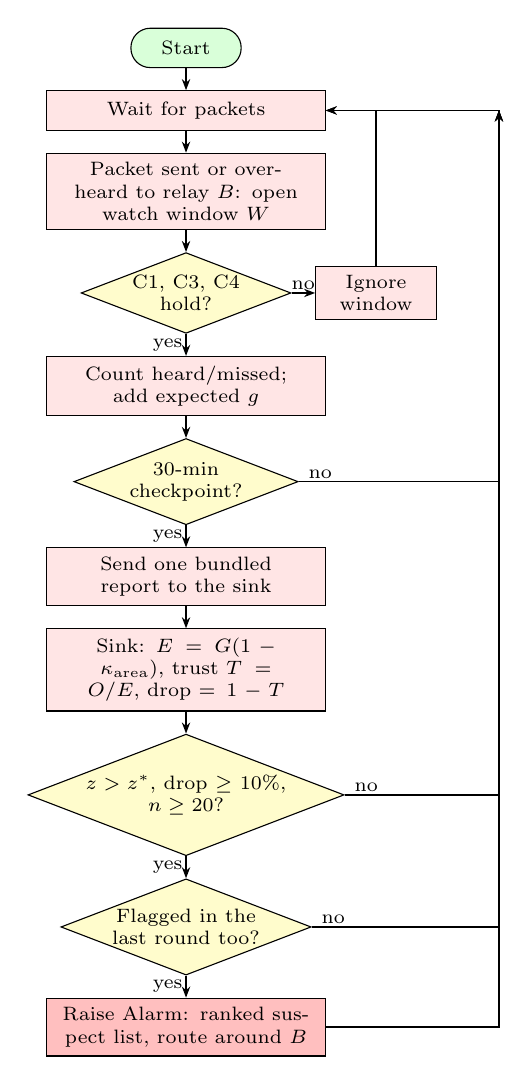
\begin{tikzpicture}[node distance=0.28cm]
\node[term] (s) {Start};
\node[proc,below=of s] (w) {Wait for packets};
\node[proc,below=of w] (o) {Packet sent or overheard to relay $B$: open watch window $W$};
\node[dec,below=of o] (obs) {C1, C3, C4\\hold?};
\node[proc,right=0.3cm of obs,text width=1.3cm] (ig) {Ignore window};
\node[proc,below=of obs] (c) {Count heard/missed; add expected $g$};
\node[dec,below=of c] (cp) {30-min\\checkpoint?};
\node[proc,below=of cp] (rep) {Send one bundled report to the sink};
\node[proc,below=of rep] (sc) {Sink: $E=G(1-\kappa_{\mathrm{area}})$, trust $T=O/E$, drop $=1-T$};
\node[dec,below=of sc] (fl) {$z>z^*$, drop $\geq$ 10\%,\\$n\geq 20$?};
\node[dec,below=of fl] (tw) {Flagged in the\\last round too?};
\node[alarm,below=of tw] (al) {Raise Alarm: ranked suspect list, route around $B$};
\draw[flow] (s)--(w); \draw[flow] (w)--(o); \draw[flow] (o)--(obs);
\draw[flow] (obs)--node[lbl,above]{no}(ig);
\draw[flow] (obs)--node[lbl,left]{yes}(c);
\draw[flow] (c)--(cp);
\draw[flow] (cp)--node[lbl,left]{yes}(rep);
\draw[flow] (rep)--(sc); \draw[flow] (sc)--(fl);
\draw[flow] (fl)--node[lbl,left]{yes}(tw);
\draw[flow] (tw)--node[lbl,left]{yes}(al);
\coordinate (back) at ($(w.east)+(2.2,0)$);
\draw[flow] (ig.north)|-(w.east);
\draw[flow] (cp.east)--node[lbl,above]{no}++(0.55,0)-|(back)--(w.east);
\draw[flow] (fl.east)--node[lbl,above]{no}++(0.55,0)-|(back);
\draw[flow] (tw.east)--node[lbl,above]{no}++(0.55,0)-|(back);
\draw[flow] (al.east)-|(back);
\end{tikzpicture}
\caption{Sequence of the detection strategy.}\label{fig:detectflow}
\end{figure}

Every 30 minutes the sink runs the detector on the latest report of every link. A relay is flagged when three conditions hold: it was judged on at least 20 windows, its estimated drop rate is at least 10\%, and its deviation $z$, the shortfall of heard forwards measured in standard deviations, is above a threshold $z^*$. The threshold is dynamic: it grows with the number of judged relays, and $z$ is first rescaled by how widely honest relays spread in the current round. When several grayholes sit in one area, they raise the area's normal loss and hide one another; the detector therefore removes relays with at least 10\% estimated drop, and confirmed suspects, from the area medians and repeats the estimate. A relay that is flagged in two rounds in a row becomes a suspect, and the sink routes traffic around it wherever another path exists.

\section{Implementation of the Grayhole Attack and Detection in UnetStack}\label{sec:impl}
The implementation uses UnetStack 7.0.0 (community edition) with Java~8. Each node runs one agent, \texttt{MonitorNode}, which generates data, relays packets, acts as a grayhole when told to, and monitors its neighbours. The acoustic channel is UnetStack's \texttt{ProtocolChannelModel} extended in \texttt{DistanceLossChannel} so that the chance of decoding a frame falls with distance as $1-0.15\,(d/1500)^2$; far links therefore lose more frames than near ones even when every node is honest. The class diagram of the implementation is given in Figure~\ref{fig:classes}.

\begin{figure*}[t]\centering
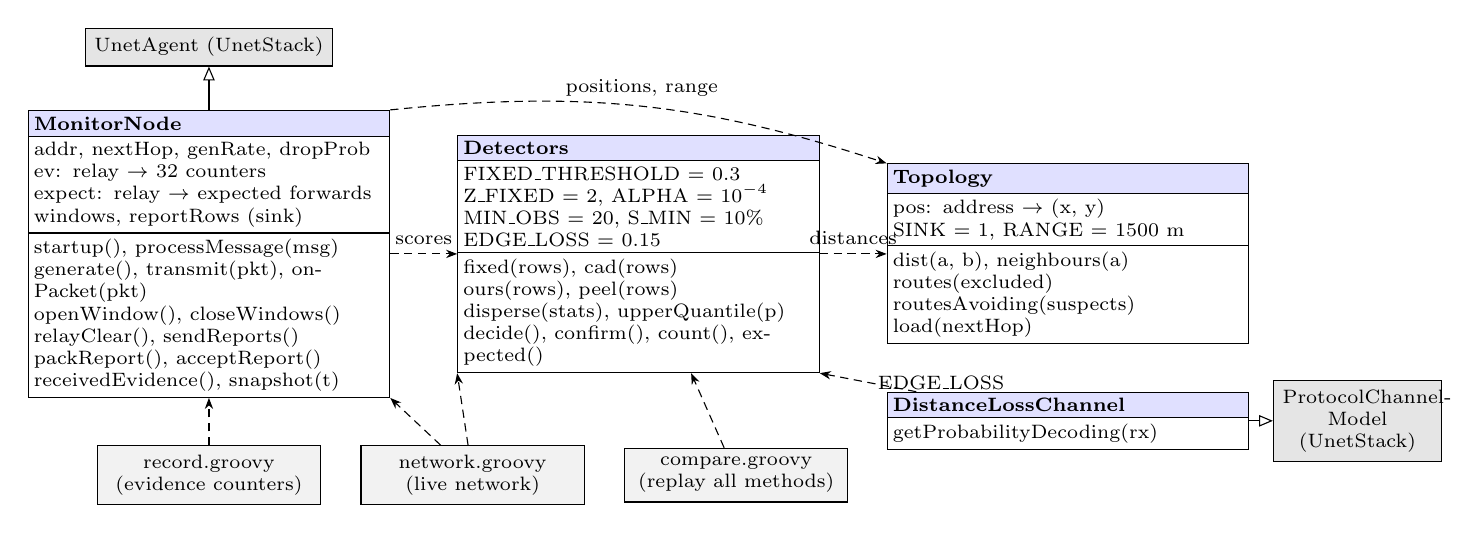
\begin{tikzpicture}[font=\scriptsize,
  cls/.style={draw,rectangle split,rectangle split parts=3,rectangle split part fill={blue!12,white,white},align=left,text width=4.45cm,inner sep=2pt},
  scr/.style={draw,fill=gray!10,align=center,text width=2.6cm,minimum height=0.55cm},
  uses/.style={-{Stealth[length=4pt]},densely dashed},
  inh/.style={-{Triangle[open,length=5pt]}}]
\node[cls] (mon) at (0,0) {\centering\textbf{MonitorNode}
\nodepart{second}addr, nextHop, genRate, dropProb\\ev: relay $\to$ 32 counters\\expect: relay $\to$ expected forwards\\windows, reportRows (sink)
\nodepart{third}startup(), processMessage(msg)\\generate(), transmit(pkt), onPacket(pkt)\\openWindow(), closeWindows()\\relayClear(), sendReports()\\packReport(), acceptReport()\\receivedEvidence(), snapshot(t)};
\node[cls,right=0.85cm of mon] (det) {\centering\textbf{Detectors}
\nodepart{second}FIXED\_THRESHOLD = 0.3\\Z\_FIXED = 2, ALPHA = $10^{-4}$\\MIN\_OBS = 20, S\_MIN = 10\%\\EDGE\_LOSS = 0.15
\nodepart{third}fixed(rows), cad(rows)\\ours(rows), peel(rows)\\disperse(stats), upperQuantile(p)\\decide(), confirm(), count(), expected()};
\node[cls,right=0.85cm of det] (top) {\centering\textbf{Topology}
\nodepart{second}pos: address $\to$ (x, y)\\SINK = 1, RANGE = 1500 m
\nodepart{third}dist(a, b), neighbours(a)\\routes(excluded)\\routesAvoiding(suspects)\\load(nextHop)};
\node[draw,fill=gray!20,above=0.55cm of mon] (ua) {UnetAgent (UnetStack)};
\node[cls,below=0.6cm of top,rectangle split parts=2] (ch) {\centering\textbf{DistanceLossChannel}
\nodepart{second}getProbabilityDecoding(rx)};
\node[draw,fill=gray!20,right=0.3cm of ch,text width=1.9cm,align=center] (pcm) {ProtocolChannel\-Model (UnetStack)};
\node[scr,below=0.6cm of mon] (rec) {record.groovy\\(evidence counters)};
\node[scr,right=0.5cm of rec] (net) {network.groovy\\(live network)};
\node[scr,right=0.5cm of net] (cmp) {compare.groovy\\(replay all methods)};
\draw[inh] (mon)--(ua);
\draw[inh] (ch)--(pcm);
\draw[uses] (mon)--node[above]{scores}(det);
\draw[uses] (det)--node[above]{distances}(top);
\draw[uses] (mon.north east)to[bend left=12]node[above]{positions, range}(top.north west);
\draw[uses] (rec)--(mon); \draw[uses] (net)--(mon.south east);
\draw[uses] (net)--(det.south west); \draw[uses] (cmp)--(det);
\draw[uses] (ch)--node[right]{EDGE\_LOSS}(det.south east);
\end{tikzpicture}
\caption{Class diagram of the implementation. Solid arrows with open heads show inheritance, dashed arrows show use.}\label{fig:classes}
\end{figure*}

\subsection{Attack Model}
The agent used has three main functions: \textbf{startup()}, \textbf{generate()} and \textbf{onPacket()}, along with a utility function \texttt{transmit(pkt)}, which sends a packet to the current next hop using a \texttt{TxFrameReq} to the physical layer. A data packet is 8 bytes long: origin, sequence number, generation time and hop count.

\subsubsection{startup()}
The role of startup() is akin to that of the main() function in any regular computer program~\cite{chitre}. It is called once when the agent starts, finds the physical-layer agent, subscribes to its notifications, and adds the behaviours that run for the rest of the simulation.
\begin{lstlisting}
startup() {
  phy = agentForService(PHYSICAL)
  subscribe(topic(phy))        // overhear every frame
  subscribe(topic(DATAGRAM))   // frames for this node
  if (genRate > 0)
    add PoissonBehavior(1/genRate) { generate() }
  add TickerBehavior(200 ms) { closeWindows() }
  add TickerBehavior(30 min) {
    snapshot(); sendReports(); onRound() }
}
\end{lstlisting}

\subsubsection{generate()}
It builds a new data packet with the node's address and the next sequence number and passes it to transmit().

\subsubsection{onPacket()}
This function carries out the attack. It is called for every packet addressed to the node. The sink records the delivery, or stores the report. Any other node forwards the packet, unless it is a grayhole and the random draw tells it to drop the packet.
\begin{lstlisting}
onPacket(pkt) {
  if (addr == SINK) {
    if (isReport(pkt)) acceptReport(pkt)
    else delivered.add(pkt)
    return
  }
  if (dropProb > 0 && random() < dropProb)
    return                     // grayhole drops it
  pkt.hops++
  transmit(pkt)                // forward to next hop
}
\end{lstlisting}

\subsection{Detection Approach}
The agent designed here has 3 primary functions for the monitor: \textbf{openWindow()}, \textbf{closeWindows()} and \textbf{relayClear()}, along with \textbf{sendReports()}. The detector itself is in the class \texttt{Detectors}, whose main function is \textbf{ours()}. Report transmissions are jittered over ten minutes to prevent packet collisions between reports.

\subsubsection{openWindow()}
When the node's own frame leaves (\texttt{TxFrameNtf}) or when it overhears a frame addressed to another node (\texttt{RxFrameNtf}), it opens a window for the relay. If a frame from relay $B$ carrying the same packet identity is overheard while the window is open, the window is marked as heard.
\begin{lstlisting}
openWindow(B, id, arrEnd, src, sender) {
  if (B == SINK || dist(addr, B) > RANGE) return
  back = dist(B, addr) / SOUND
  windows[B:id] = [heard: false, src, sender,
    I: [arrEnd - FRAME, arrEnd],
    W: [arrEnd + back, arrEnd + FWD_WAIT + FRAME + back]]
}
\end{lstlisting}

\subsubsection{closeWindows()}
Every 200~ms it closes the windows that have ended, checks the conditions and adds the outcome to one of 32 counters, so that every method can later be judged on the same evidence. The counter index keeps whether the monitor was the sender, which conditions failed and whether the forward was heard.
\begin{lstlisting}
for (w in windows where now > w.W.end + 50 ms) {
  c13 = !overlaps(myTx, w.W) && !overlaps(heardTx[B], w.I)
  c2  = !overlaps(badFrames, w.W)   // kept, not used
  c4  = relayClear(w)
  i = idx(w.sender, c13, c2, c4, w.heard)
  ev[B][i]++
  expect[B][i] += (1 - e(d(src,B))) * (1 - e(d(B,addr)))
  remove(w)
}
\end{lstlisting}

\subsubsection{relayClear()}
It checks C4. A frame sent by node $C$ during $[t_0,t_1]$ is at $B$ during $[t_0,t_1]$ shifted by $d(C,B)/c$. If such a known frame overlaps $I_B$, the packet may have collided at $B$ and the window is not observable.
\begin{lstlisting}
relayClear(w) {
  for (C, frames in heardTx + [addr: myTx]) {
    if (C == w.src || C == B || dist(C, B) > RANGE) continue
    shift = dist(C, B) / SOUND
    if (any frame f: f + shift overlaps w.I)
      return false             // possible collision at B
  }
  return true
}
\end{lstlisting}

\subsubsection{sendReports()}
At each checkpoint the monitor freezes its counters and bundles them into one report frame: a 12-byte header and one 17-byte entry per watched relay (relay, windows, misses and expected forwards), at most six entries in the 128-byte frame. The report travels to the sink over the same lossy network as the data, and can be lost or dropped by a grayhole. The sink keeps the latest delivered report of every link; since the counters are cumulative, a lost report only delays evidence.

\subsubsection{ours()}
This is the detector at the sink. The following are the parameters used by ours():
\begin{itemize}
\item \textbf{MIN\_ROW} -- a link joins the estimate with at least 5 windows.
\item \textbf{MIN\_OBS} -- a relay is judged on at least 20 windows.
\item \textbf{S\_MIN} -- minimum estimated drop rate to flag, 10\%.
\item \textbf{ALPHA} -- false-alarm setting, $10^{-4}$, chosen on separate tuning networks.
\item \textbf{CHI2\_MEDIAN} -- 0.455, the median of $z^2$ for an honest relay, used to measure the spread of a round.
\end{itemize}
Given below is the gist of the UnetStack code for the mechanism.
\begin{lstlisting}
for (link i with n_i >= MIN_ROW)
  kappa_i = max(0, 1 - O_i/G_i)  // unexplained loss
zone = near / medium / far tertile of link distance
for (relay B) {
  kArea = median(kappa of OTHER relays' links in zone)
  E_i = G_i * (1 - kArea)    // expected forwards
  trust = sum(O_i) / sum(E_i); drop = 1 - trust
  z = (sum E - sum O) / sqrt(sum E_i (1 - E_i/n_i))
}
z = z / sqrt(phi)            // spread of this round
zStar = upperQuantile(ALPHA / judgedRelays)
flag B if n >= MIN_OBS && drop >= S_MIN && z > zStar
\end{lstlisting}
The function \textbf{peel()} repeats ours() at most three times, leaving out relays with at least 10\% estimated drop and confirmed suspects from the area medians, until the set is stable. This code repeats every 30 minutes till there is no more transmission.

\subsubsection{onRound()}
At the sink, after every round, the flagged set is confirmed and the routes are updated. A suspect stays one until the administrator reviews it.
\begin{lstlisting}
onRound(t) {
  rows = receivedEvidence()   // delivered only
  flagged = peel(rows, ALPHA, suspects).flagged
  suspects += flagged.intersect(lastFlagged)
  lastFlagged = flagged
  if (suspects changed)
    nextHop = routesAvoiding(suspects)
}
\end{lstlisting}
The function \texttt{routesAvoiding()} gives every node a shortest route that avoids the suspects; a node with no such route keeps its old route, since a lossy path is better than none. The two baselines use exactly the same agent, reports, confirmation and response, so only the detection rule differs.

\begin{figure*}[t]\centering
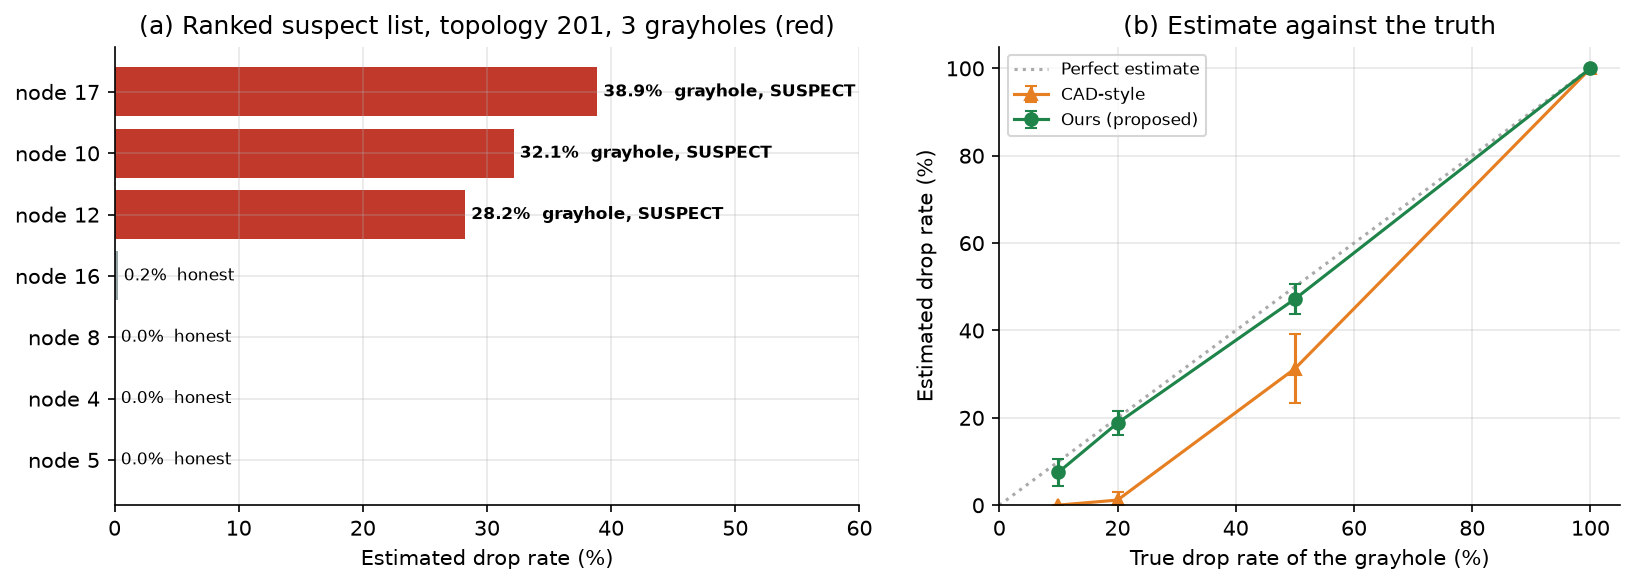
\includegraphics[width=0.85\textwidth]{figs/fig4_suspect_list.png}
\caption{(a) Ranked suspect list for test network 201 with three grayholes; (b) estimated against true drop rate.}\label{fig:suspect}
\end{figure*}

\begin{figure*}[t]\centering
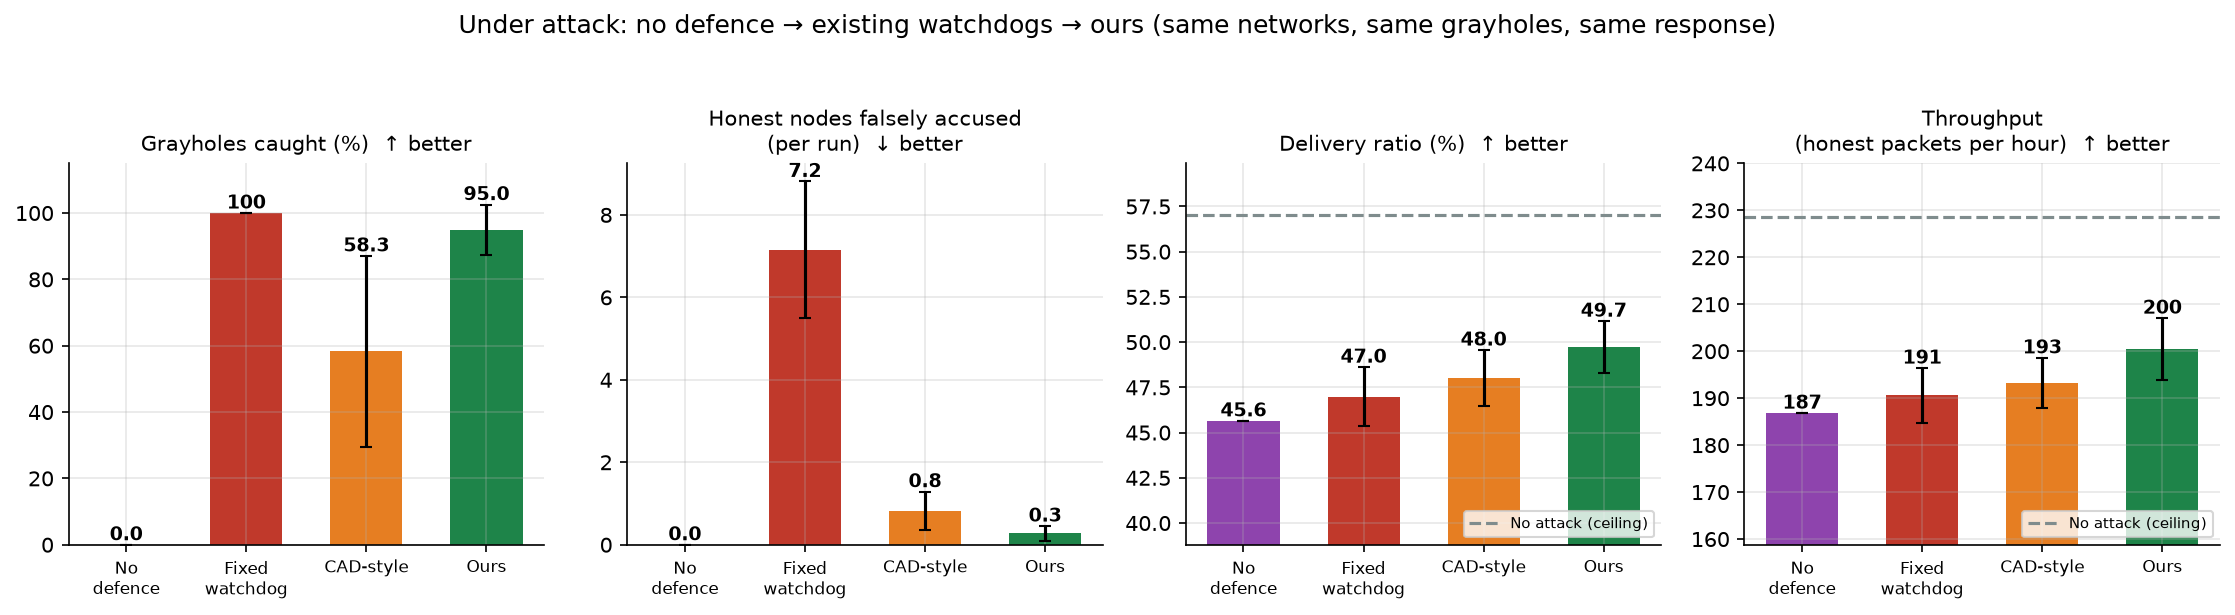
\includegraphics[width=0.9\textwidth]{figs/fig1_before_after.png}
\caption{Baseline vs proposed in the live network: grayholes caught, honest nodes accused, delivery ratio and throughput (12~h, ten test networks). The dashed line is the same networks without attack.}\label{fig:before}
\end{figure*}

\begin{figure*}[t]\centering
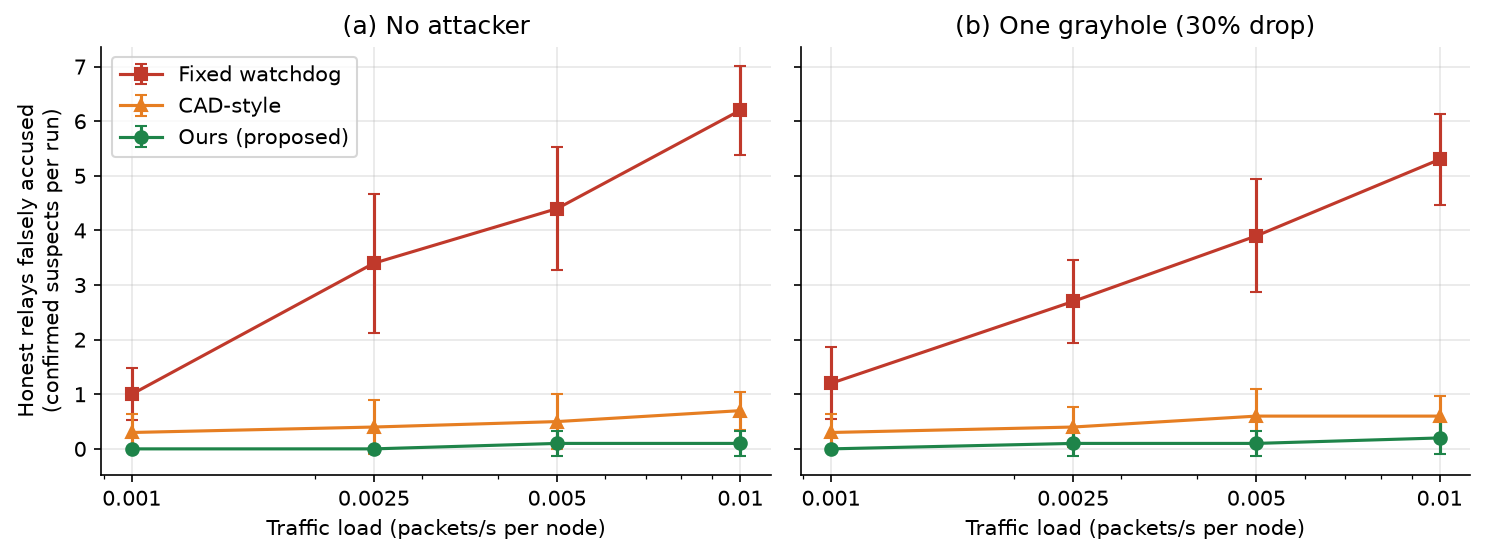
\includegraphics[width=0.9\textwidth]{figs/fig2_false_accusations.png}
\caption{Honest relays falsely accused per run for different traffic loads, each method with its own rule (6~h, ten test networks).}\label{fig:false}
\end{figure*}

\begin{figure*}[t]\centering
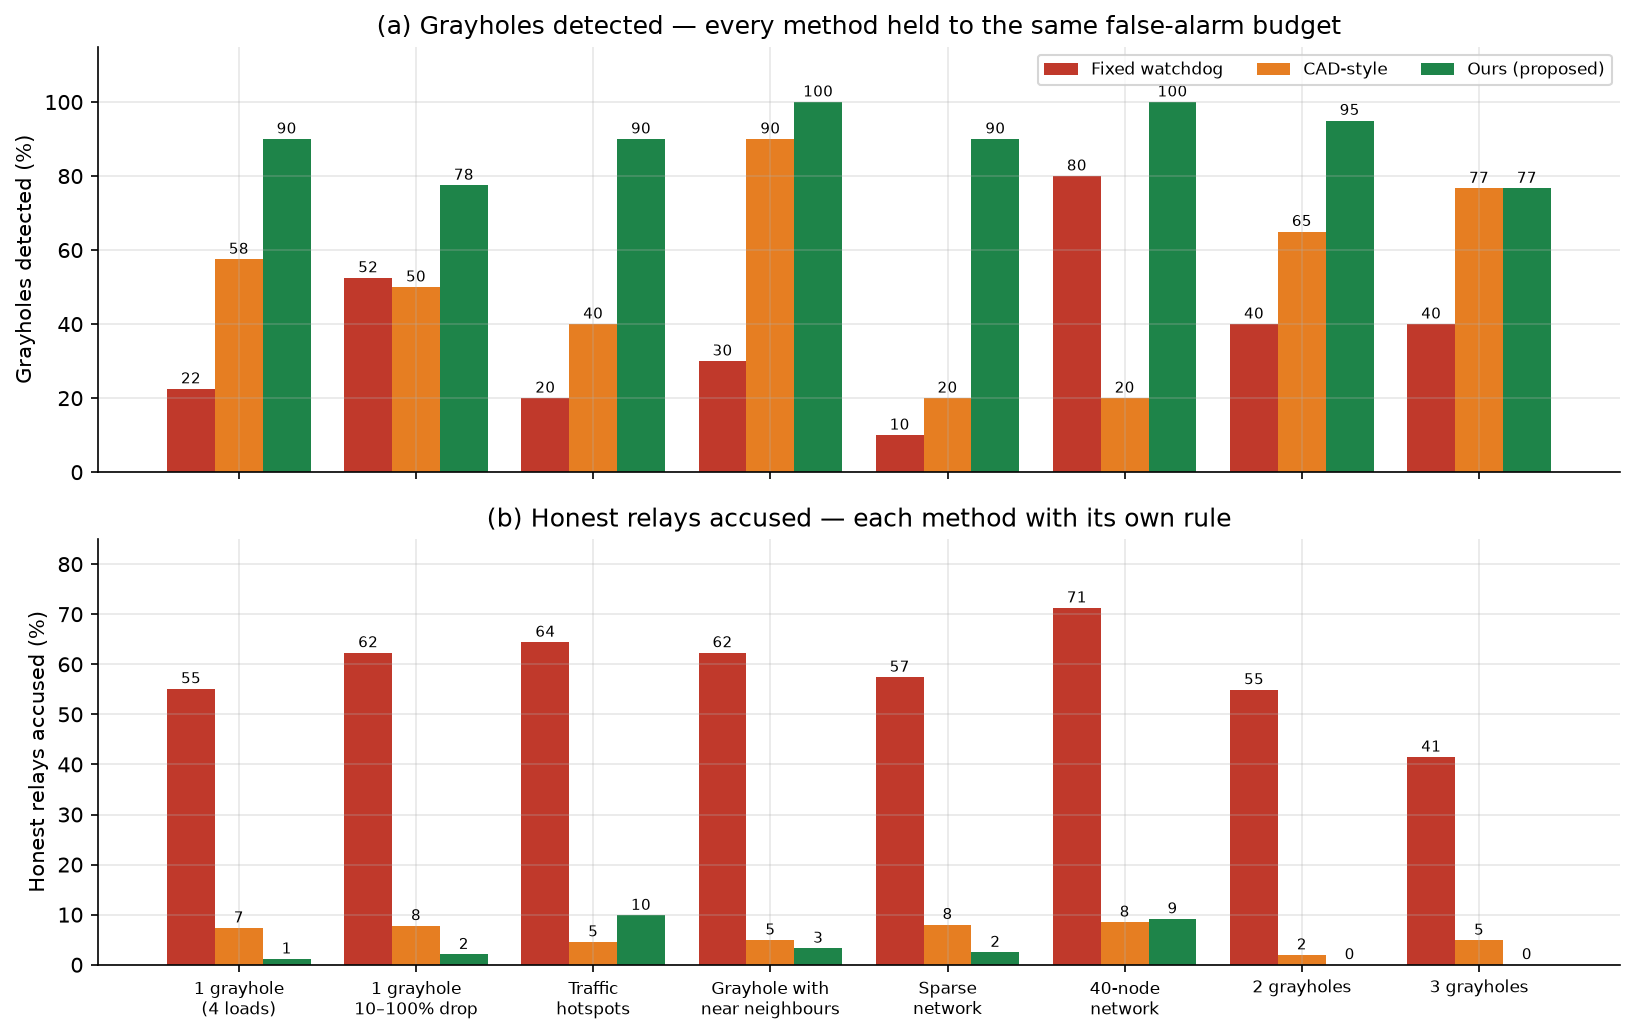
\includegraphics[width=0.9\textwidth]{figs/fig3_detection.png}
\caption{(a) Grayholes detected with all methods held to the same false-alarm budget; (b) honest relays accused with each method's own rule.}\label{fig:fair}
\end{figure*}

\begin{figure*}[t]\centering
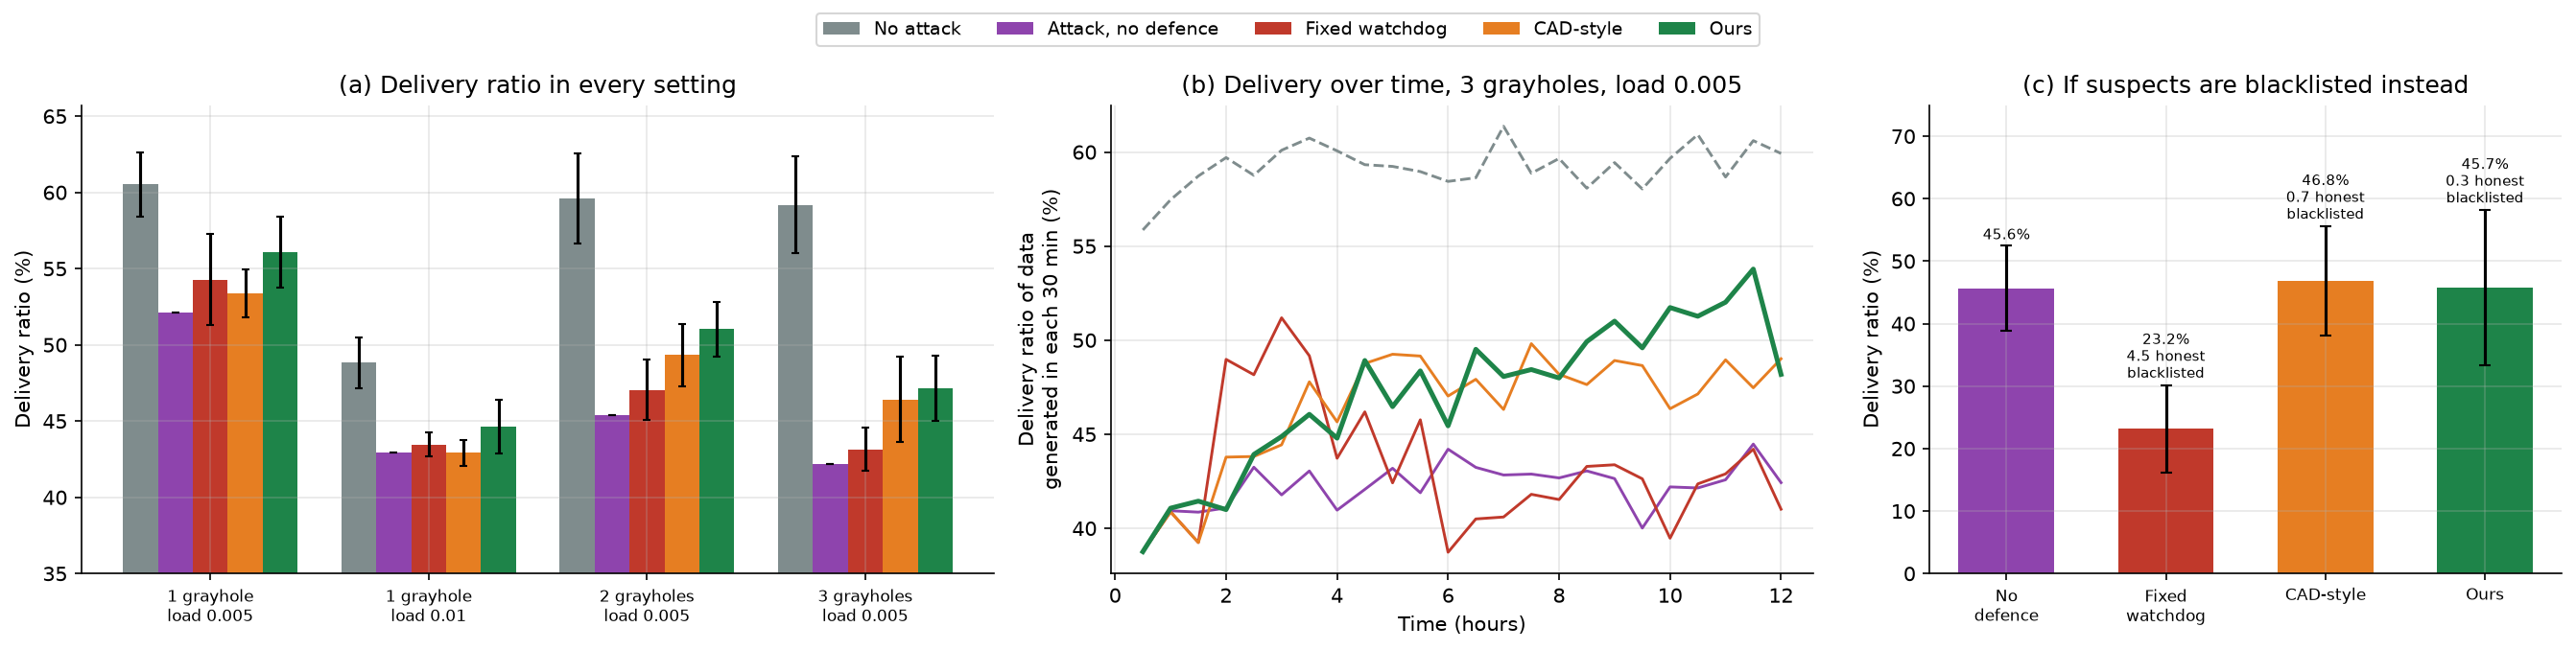
\includegraphics[width=0.9\textwidth]{figs/fig5_network_performance.png}
\caption{Live network: (a) delivery ratio per setting, error bars are paired 95\% intervals against no defence; (b) delivery over time with three grayholes; (c) delivery when suspects are blacklisted.}\label{fig:network}
\end{figure*}

\section{Results}\label{sec:results}
All experiments run in one pipeline (\texttt{run.sh}): \texttt{record.groovy} simulates the networks and stores every monitor's counters, \texttt{compare.groovy} replays the sink's decisions for every method on exactly the same counters, \texttt{network.groovy} runs the live network in which reports, detection and rerouting all happen inside the simulation, and a Python script draws the graphs. The simulation parameters are as follows:
\begin{itemize}
\item \textbf{Network} -- 20 sensors and one sink in 4~km~$\times$~4~km, range 1500~m, sound speed 1500~m/s; a 40-node and a sparse variant.
\item \textbf{Traffic} -- 0.001 to 0.01 packets/s per sensor; 0.005 unless stated.
\item \textbf{Grayholes} -- the 1, 2 or 3 busiest relays, dropping 30\% of relayed packets (10--100\% in a sweep).
\item \textbf{Networks} -- thresholds tuned on topologies 101--106 only; results on test topologies 201--210.
\item \textbf{Duration} -- 6~h recorded runs, 12~h live-network runs, one decision every 30~min.
\item \textbf{Baselines} -- fixed watchdog (miss rate $>30\%$) and CAD-style ($z>2$).
\end{itemize}

\subsection{Attack Model}
The first subsection examines the performance of the attack model. The strength of the attack is controlled by the number of grayholes, each dropping 30\% of the packets it should forward. Figure~\ref{fig:attack} shows a graph showing the delivery ratio lost to the attack for different numbers of grayholes, measured against the same network without attack and without any defence. Each value is the average of 10 test networks. Each run lasted 12 hours, in which every sensor sent about 216 packets.

\begin{figure}[H]\centering
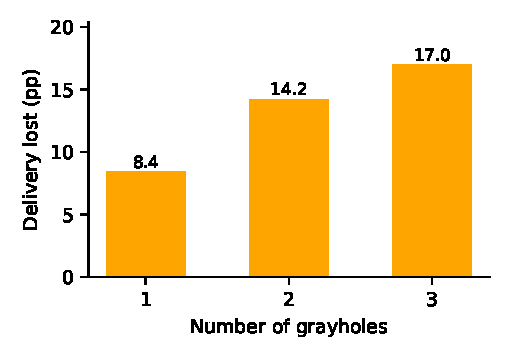
\includegraphics[width=0.65\columnwidth]{figs/attack.pdf}
\caption{Delivery lost for different numbers of grayholes (pp: percentage points of honest packets delivered).}\label{fig:attack}
\end{figure}

It can be seen that the higher the number of grayholes, the more of the honest traffic is lost: 8.4, 14.2 and 17.0 percentage points of delivery for one, two and three grayholes. Furthermore, the loss grows more slowly with each added grayhole, since the busiest relay is attacked first and the later ones carry less traffic.

\subsection{Detection Approach}
Coming to the detection approach, the first question is whether the grayholes are found at all. Figure~\ref{fig:detected} shows the fraction of grayholes confirmed as suspects by the end of a 6-hour run, and Figure~\ref{fig:dtime} the time at which every grayhole of a run had been confirmed, averaged over the runs in which this happened. Due to the random nature of packet drops and collisions, the time differs from run to run; since a relay needs two flagged rounds in a row, the earliest possible confirmation is after 60 minutes.

\begin{figure}[H]\centering
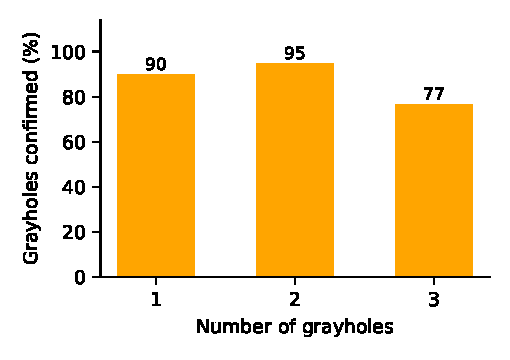
\includegraphics[width=0.65\columnwidth]{figs/detected.pdf}
\caption{Grayholes confirmed for different numbers of grayholes.}\label{fig:detected}
\end{figure}

The detector confirmed 90\% of single grayholes, 95\% of grayholes in networks with two and 77\% in networks with three. The detection time roughly rises from 97 to 140 minutes as grayholes are added, since several grayholes raise the normal loss of their area and hide one another until the baseline has been cleaned.

\begin{figure}[H]\centering
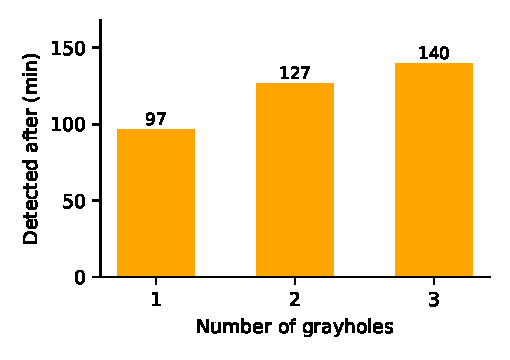
\includegraphics[width=0.65\columnwidth]{figs/detect_time.pdf}
\caption{Detection time for different numbers of grayholes.}\label{fig:dtime}
\end{figure}

Figure~\ref{fig:suspect}(a) is the list the administrator receives for the network of Figure~\ref{fig:topology}. The three grayholes rank first, with estimated drop rates of 38.9\%, 32.1\% and 28.2\%, and are confirmed; every honest relay is estimated at 0--0.2\%. Figure~\ref{fig:suspect}(b) shows that the estimate follows the true drop rate: 7.6, 18.8 and 47.2\% for true rates of 10, 20 and 50\%.

\subsection{Comparison with the Baselines}
Figure~\ref{fig:before} compares the baseline and the proposed approach in the live network, pooled over every setting. Under attack the fixed watchdog catches every grayhole only by accusing 7.2 honest nodes per run, and routing around them costs most of what it gains: delivery rises only from 45.6\% to 47.0\%. The CAD-style detector accuses fewer honest nodes (0.8) but misses 42\% of the grayholes. Ours catches 95\% of the grayholes while accusing 0.3 honest nodes per run, and gives the highest delivery ratio (49.7\%) and throughput (200.5 against 186.8 packets per hour without defence).

The reason is shown in Figure~\ref{fig:false}. With no attacker at all, the fixed watchdog accuses 1.0 honest relay per run at the lowest load and 6.2 at the highest, because collisions and half-duplex deafness grow with traffic and are counted as drops. The CAD-style detector accuses 0.3--0.7, and ours 0--0.1.

Figure~\ref{fig:fair} is a fair contest: every method's threshold is tuned on the separate tuning networks so that at most 5\% of honest relays are accused without an attacker. Ours then detects 90\% of single grayholes (CAD-style 58\%, fixed 22\%), 95\% with two grayholes (65\%, 40\%) and 77\% with three (77\%, 40\%). With their own rules, the fixed watchdog reaches 100\% only by accusing 41--71\% of honest relays. In the traffic-hotspot and 40-node networks, ours accuses about 10\% of honest relays, which is more than the fixed watchdog at the same budget.

Figure~\ref{fig:network} breaks the live-network delivery down by setting. Ours has the highest delivery in all four settings. Compared with no defence on the same networks it gains 4.0, 1.7, 5.6 and 4.9 percentage points, and compared with the fixed watchdog 4.0 points with two and with three grayholes. Against the CAD-style detector ours is ahead by 0.7--2.7 points, which is within the uncertainty. When suspects are blacklisted instead of avoided, every honest node the fixed watchdog accuses is lost together with the nodes behind it, and its delivery falls to 23.2\%, against 45.6\% without defence.

Finally, each part of the method was removed in turn at the same budget. Without baseline cleaning, detection with three grayholes falls from 23 of 30 to 17 of 30. Without the observability filter, detection is similar, but honest accusations rise slightly (1.5\% against 1.1\% in the load sweep); with two-round confirmation in place, the filter's contribution in these networks is therefore small.

\section{Conclusions and Future work}\label{sec:conclusion}
We have demonstrated a grayhole attack model as well as an observability-aware, trust-based detection strategy for underwater acoustic networks, implemented in UnetStack and compared with a fixed-threshold watchdog and a CAD-style detector. A performance evaluation of all of them has been done and the results shown in graphs: the detector caught 95\% of the grayholes while accusing 0.3 honest nodes per run, against 7.2 for the fixed watchdog, and gave the highest delivery ratio.

The limitations of this paper are as follows. The topologies are static, node positions and the distance--loss curve are assumed known, and every monitor reports truthfully. The baselines are adaptations, not full reproductions of the published systems, and route updates are free in the simulation. In hotspot and 40-node networks ours accuses about 10\% of honest relays.

Future implementations can work on making the detector robust to monitors that send false reports, and to mobile nodes and location errors. Work can be done to learn the loss curve online instead of assuming it. Finally, the above approach is only a detection and avoidance scheme. Work can be done to implement an isolation approach that will run on UnetStack without cutting off the nodes behind a grayhole.

\section*{Acknowledgment}
The authors thank the course staff of CS301 and Mohit sir, Department of Computer Science and Engineering, NITK Surathkal, for their guidance.

\begin{thebibliography}{12}
\bibitem{akyildiz} I. F. Akyildiz, D. Pompili, and T. Melodia, ``Underwater acoustic sensor networks: research challenges,'' \emph{Ad Hoc Networks}, vol.~3, no.~3, pp.~257--279, 2005, doi: 10.1016/j.adhoc.2005.01.004.
\bibitem{karlof} C. Karlof and D. Wagner, ``Secure routing in wireless sensor networks: attacks and countermeasures,'' \emph{Ad Hoc Networks}, vol.~1, no.~2--3, pp.~293--315, 2003, doi: 10.1016/S1570-8705(03)00008-8.
\bibitem{domingo} M. C. Domingo, ``Securing underwater wireless communication networks,'' \emph{IEEE Wireless Communications}, vol.~18, no.~1, pp.~22--28, 2011, doi: 10.1109/MWC.2011.5714022.
\bibitem{jiang} S. Jiang, ``On securing underwater acoustic networks: a survey,'' \emph{IEEE Communications Surveys \& Tutorials}, vol.~21, no.~1, pp.~729--752, 2019, doi: 10.1109/COMST.2018.2864127.
\bibitem{marti} S. Marti, T. J. Giuli, K. Lai, and M. Baker, ``Mitigating routing misbehavior in mobile ad hoc networks,'' in \emph{Proc. 6th ACM MobiCom}, 2000, pp.~255--265, doi: 10.1145/345910.345955.
\bibitem{shila} D. M. Shila, Y. Cheng, and T. Anjali, ``Mitigating selective forwarding attacks with a channel-aware approach in WMNs,'' \emph{IEEE Transactions on Wireless Communications}, vol.~9, no.~5, pp.~1661--1675, 2010, doi: 10.1109/TWC.2010.05.090700.
\bibitem{hanTrust} G. Han, J. Jiang, L. Shu, and M. Guizani, ``An attack-resistant trust model based on multidimensional trust metrics in underwater acoustic sensor network,'' \emph{IEEE Transactions on Mobile Computing}, vol.~14, no.~12, pp.~2447--2459, 2015, doi: 10.1109/TMC.2015.2402120.
\bibitem{liu} C. Liu, J. Ye, F. An, and W. Jiang, ``An adaptive trust evaluation model for detecting abnormal nodes in underwater acoustic sensor networks,'' \emph{Sensors}, vol.~24, no.~9, art.~2880, 2024, doi: 10.3390/s24092880.
\bibitem{hanRouting} D. Han, X. Du, L. Wang, X. Liu, and X. Tian, ``Trust-aware and fuzzy logic-based reliable layering routing protocol for underwater acoustic networks,'' \emph{Sensors}, vol.~23, no.~23, art.~9323, 2023, doi: 10.3390/s23239323.
\bibitem{brc} B. R. Chandavarkar and N. Suresh, ``Demonstration of selective forwarding attack and detection mechanism in UnetStack3,'' in \emph{Proc. 12th Int. Conf. Computing Communication and Networking Technologies (ICCCNT)}, 2021, pp.~1--6, doi: 10.1109/ICCCNT51525.2021.9580125.
\bibitem{chitre} M. Chitre, R. Bhatnagar, and W.-S. Soh, ``UnetStack: an agent-based software stack and simulator for underwater networks,'' in \emph{Proc. IEEE OCEANS}, St. John's, 2014, doi: 10.1109/OCEANS.2014.7003044.
\bibitem{unet} UnetStack, ``Unet handbook: physical service,'' \url{https://unetstack.net/handbook/305_phy.html}, accessed 12 Oct. 2026.
\end{thebibliography}

\end{document}
